%!TEX root =  ..\ekg_7_projektbericht.tex

%PCB Design

\subsection{Platinendesign}

Für das Zeichnen von Schaltplänen sowie dem Layouten der Platine wird das Programm Altium Designer verwendet. Es beinhaltet eine übersichtliche Benutzeroberfläche und zahlreiche Features wie PCB-Design in nativem 3D, interaktives Routing, hierarchische Designs, einheitliche Bibliothekenverwaltung, integrierte SPICE Simulationen und zahlreiche Export-Möglichkeiten in einem Tool. 

%TODO Abkürzungen ins Abkürzungsverzeichnis schreiben

\subsubsection{Erstellung von Bibliotheken}
Da in der integrierten Datenbank von Altium Designer nicht alle benötigten Bauteile enthalten sind, müssen diese zunächst von Hand angelegt werden. Dieser Prozess gliedert sich in drei Schritte:

\begin{enumerate}
\item Erstellung des Schaltzeichens: Hierbei wird mithilfe von geometrischen Formen ein Symbol des Bauteils erstellt, welches schematisch seine Funktion widerspiegelt. Idealerweise dient dafür ein Symbol des Herstellers als Vorlage. Hierbei müssen bereits die Ein- und Ausgangspins des Bauteils festgelegt werden, da nur dort später Leitungen angeschlossen werden können. Den Pins wird eine Nummer zugewiesen, welche später einem Pad des Footprints entspricht.

\item Erstellung des Footprints: Für jeden Pin des Bauteils muss ein Pad auf dem PCB erstellt werden, auf welchem das Beinchen später aufliegt und verlötet wird. Dabei ist auf eine ausreichende Größe des Pads zu achten, um eine sichere Lötstelle zu gewährleisten. Es empfiehlt sich, die Pads länger als nötig zu gestalten, wenn im Nachgang noch Bauteile per Hand verlötet werden sollen. Idealerweise verwendet das Bauteil einen Standard-Footprint, welchen es bereits als Vorlage gibt. 

\item Hinzufügen eines 3D Modells: Um die Platine später in 3D zu bearbeiten und vollständig zu exportieren, werden jedem Bauteil dreidimensionale Modelle hinzugefügt. Dies ist in Altium durch das Einfügen einer .step Datei möglich. Diese muss im Anschluss noch genau auf dem Footprint ausgerichtet werden.
\end{enumerate}

\subsubsection{Zeichnen des Schaltplans}
Der Schaltplan wird auf Basis vorangegangener Versuche erstellt. Sobald eine Baugruppe erfolgreich getestet ist, wird sie in den Schaltplan integriert. Vor dem Anlegen der einzelnen Seiten wird eine Vorlage erstellt, welche eine einheitliche Form des Schaltplans gewährleistet und Informationen wie Projektname, Ersteller oder Revisionsnummer vermittelt. Der Schaltplan ist auf vier Seiten aufgeteilt:

\begin{enumerate}
\item Power Supply
\item MCU
\item Filterung
\item Peripherie
\end{enumerate}

Die Nummerierung von Seiten und Bauteilen wurde so konfiguriert, dass diese automatisch durch Altium erfolgt. Der Schaltplan ist in funktionale Blöcke untergliedert, welche mit einem kurzen Kommentar beschriftet sind. Dies erleichtert die Übersichtlichkeit (Abbildung \ref{fig:sch_ps}).

\begin{figure} [!h]
	%\centering
	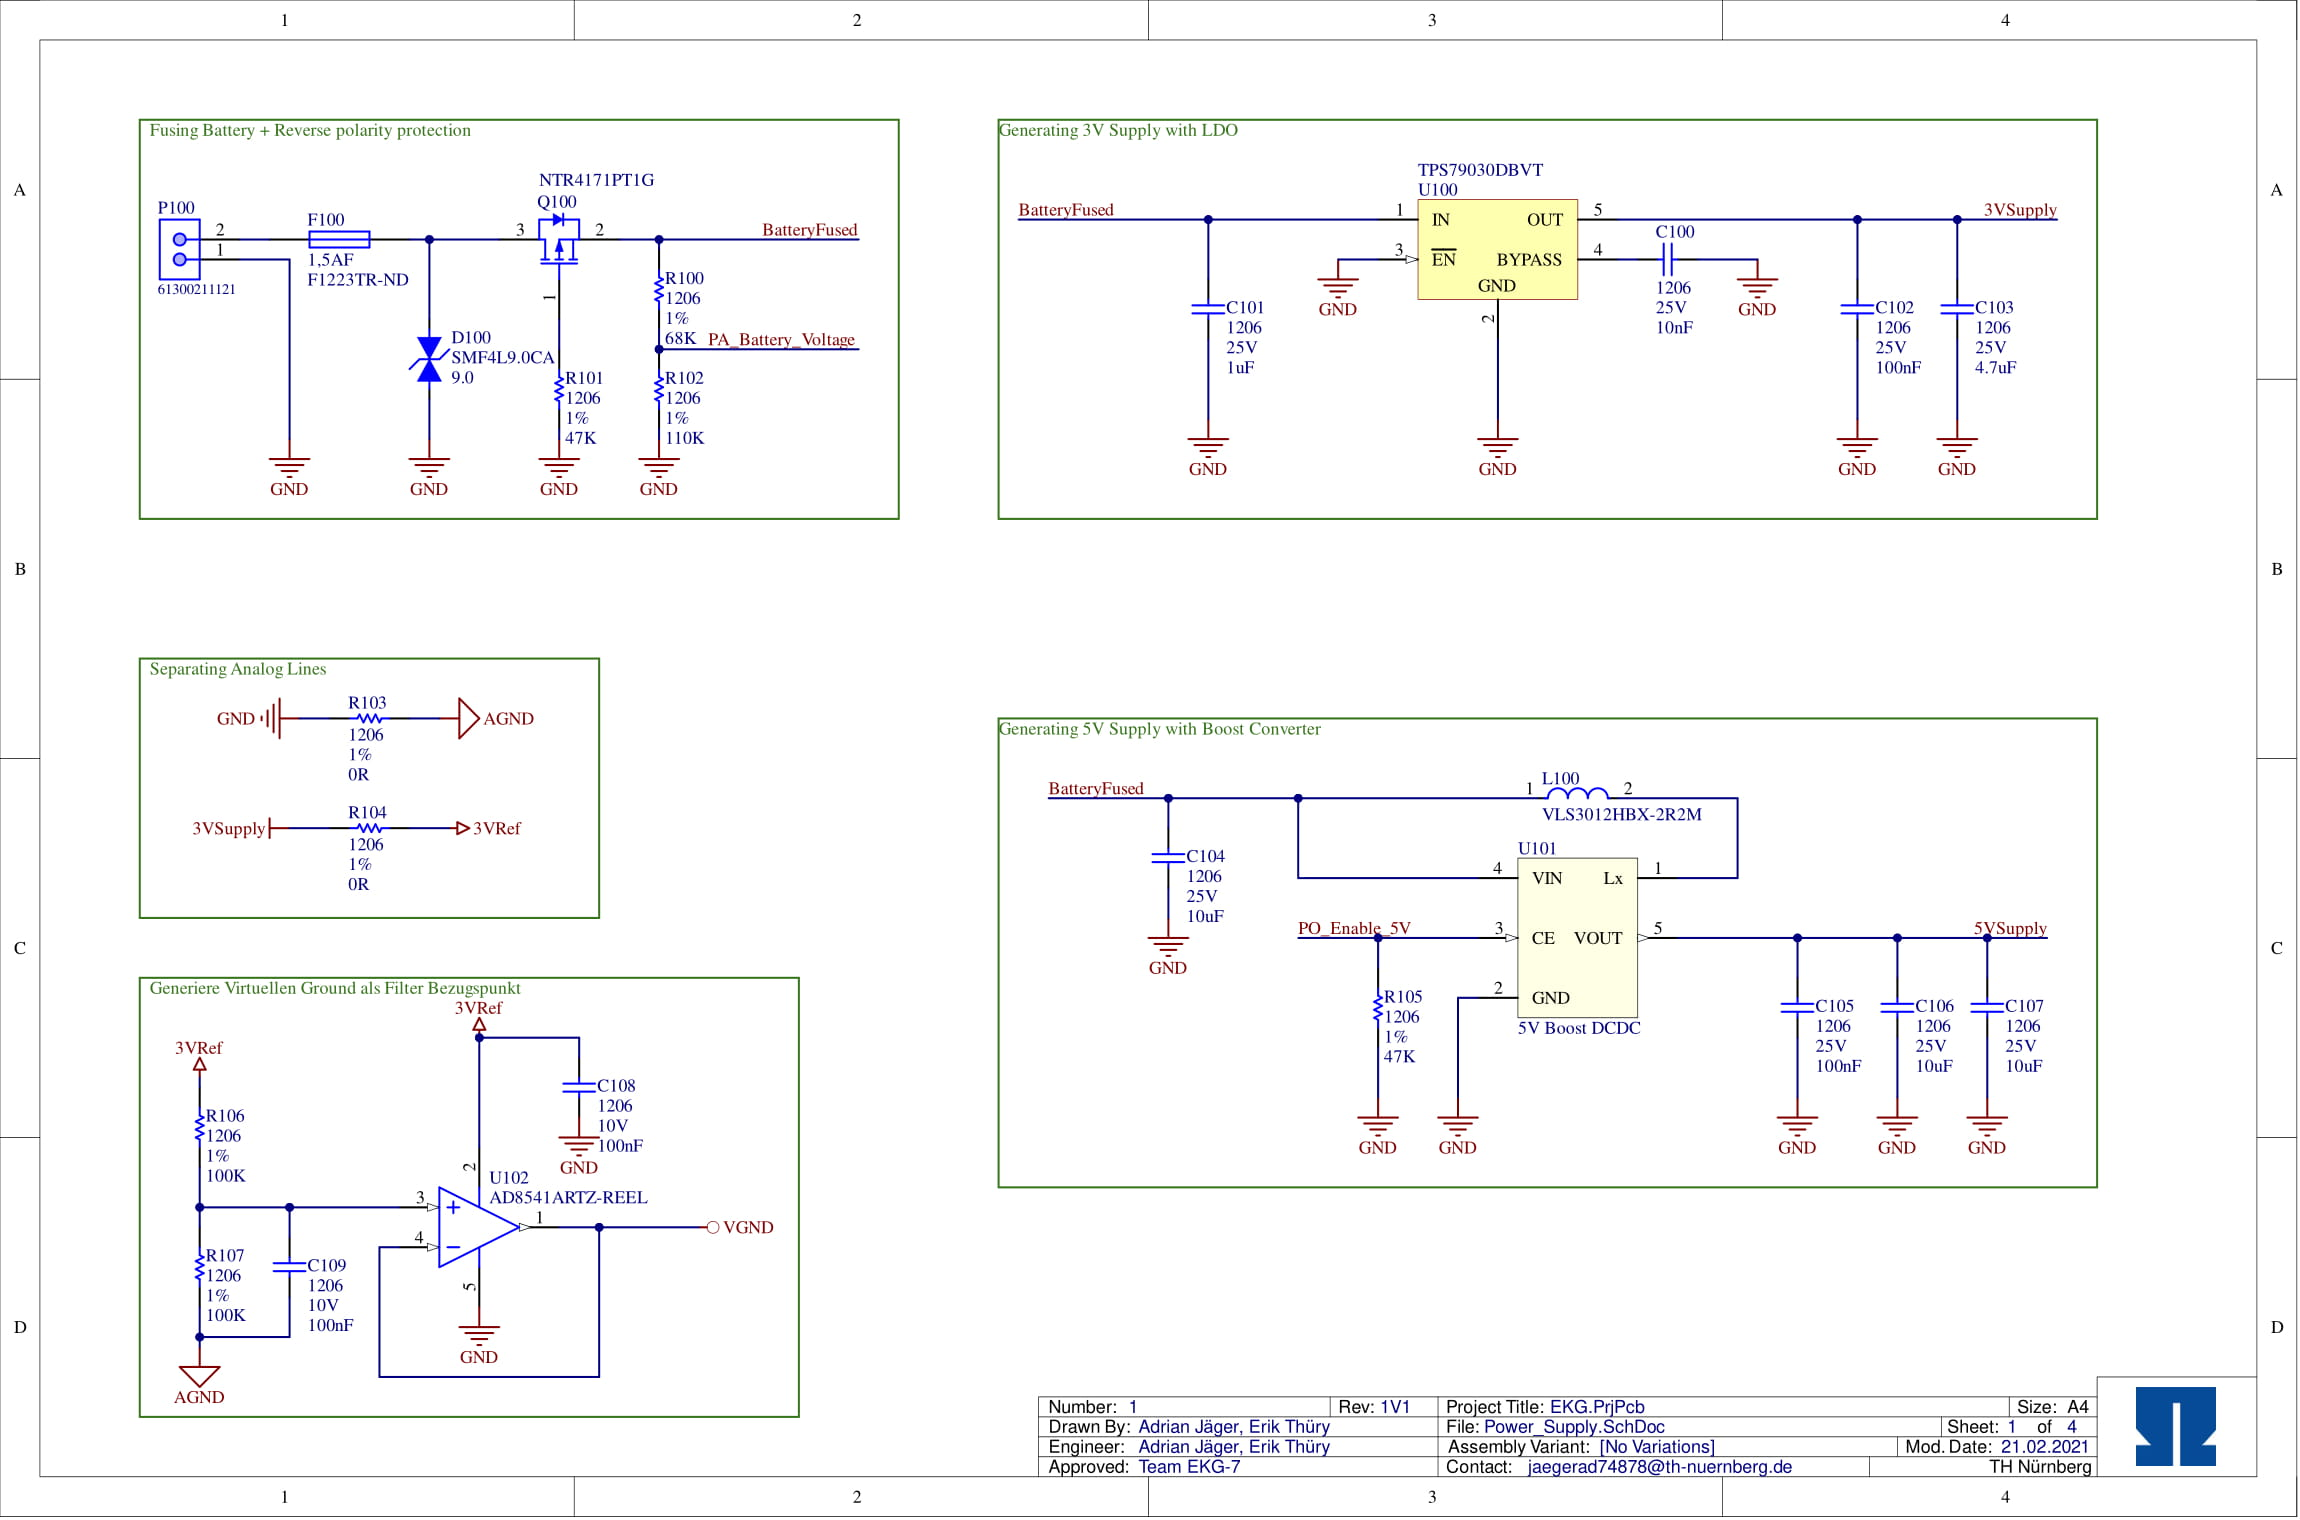
\includegraphics[width=\textwidth] {Schematics_EKG_2021-02-21_Power_Supply}
	\caption{Schaltplan Seite Power Supply}
	\label{fig:sch_ps} 
\end{figure}

Weiterhin werden Kondensatoren parallel zu den Versorgungsanschlüssen sämtlicher ICs eingeplant. Dies verhindert, dass sich Schwankungen in der Versorgungsspannung auf den IC und Lastwechsel des ICs auf die Versorgungsspannung auswirken.

\subsubsection{Platzieren der Komponente}
Nach dem Abschluss des Schaltplans kann mit dem Layout der Platine begonnen werden. Hierfür wird zunächst in Absprache mit dem Gehäuseverantwortlichen eine Maximalgröße der Platine festgelegt. Die Maße werden im \textit{Board-Planning-Mode} des neu erstellten PCB-Dokuments in Altium Designer eingetragen.

Für die Platzierung wird zunächst eine grobe Skizze auf Papier erstellt. Damit wird bereits jeder Baugruppe ein Raum auf der Platine zugewiesen, von welchem aus alle Verbindungen zu anderen Baugruppen gut erreichbar sind. 

Die MCU rückt dabei in den Mittelpunkt, da von ihr aus Verbindungen zu allen Baugruppen bestehen. Bei ihr ist darauf zu achten, das sämtliche vom Hersteller geforderten Bypass-Kondensatoren so nah wie möglich an den entsprechenden Pins platziert werden. Selbiges gilt für den externen Hochfrequenz-Schwingquarz, dessen Zuleitungen ebenfalls nur kurze Distanzen überbrücken sollten.

Die Absicherung der Spannungsversorgung ist in unmittelbarer Nähe zum Anschluss an die Batterie zu platzieren. Der 3D-Modus ist beim Platzieren von Bauteilen hilfreich um die Platzverhältnisse besser einzuschätzen.


\subsubsection{Routing}
Zum Routen wird das interaktive Routing Tool von Altium Designer verwendet. Dort werden zunächst die Design-Rules anhand der Vorgaben des Platinenfertiger Multi Circuit Boards angepasst.

Als Leiterbahnbreite werden 0,3 mm festgelegt, was ausreichend ist um selbst die höchsten zu erwartenden Ströme dauerhaft ohne gefährliche Temperaturerhöhung zu tragen. Diese Breite wird ebenso für unbelastete Signalleitungen verwendet, um bei eventuellen Lötarbeiten mehr Stabilität zu bieten. Als Größe für die Vias kommt einheitlich ein Standardvia (Lochdurchmesser 0,3 mm, Ringdurchmesser 0,65 mm) zum Einsatz. Das verringert die Werkzeugkosten des Herstellers. %TODO Quelle https://www.4pcb.com/trace-width-calculator.html

Um höchstmögliche Präzision und Störfreiheit für die Analogmessung zu ermöglichen, wird für deren Versorgung ein Sternpunkt festgelegt, welcher mit Konfigurationswiderständen vom Rest der Schaltung trennbar ist. Von diesem Sternpunkt aus wird auch die Vergleichsspannung des ADCs der MCU bedient. Auf den Leiterbahnen ist somit kein Spannungsfall oder Rauschen durch Ströme anderer Baugruppen, welche die Messung beeinflussen könnten. 

Abschließend werden Massepolygone auf das Top- und Bottom-Layer gelegt, um die Stabilität der Platine zu erhöhen und für eine verbesserte Ground-Anbindung zu sorgen. Um den Sternpunkt damit nicht zu verändern, wird für den Analogbereich ein separates Polygon verwendet.

%TODO Bild von Platine einfügen


\subsubsection{Fertigung und Bestückung}
Bevor die Platine bestellt werden kann, muss ein Design-Rule-Check (DRC) durchgeführt werden. Hierbei wird überprüft, ob die Platine alle vorgegebenen Design-Rules erfüllt. Nach der Korrektur aller Fehler werden die Gerber-Dateien automatisch mit Altium generiert und an den Hersteller versendet.
Zum Bestücken wird ein Halbautomat verwendet, welcher die Platzierung der Bauteile durch eine manuell bedienbare Saugspitze deutlich erleichtert. Die Platine mit platzierten Bauteilen durchläuft anschließend den Reflow-Ofen und wird unter dem Mikroskop auf eventuelle Lötbrücken überprüft.

\subsubsection{Inbetriebnahme}
Bei der ersten Inbetriebnahme sollte der Strom zunächst durch ein Labornetzteil begrenzt werden. Nach dem Anschluss der EKG Platine wurde festgestellt, dass diese einen Kurzschluss mit Dioden-Charakteristik verursacht. Sobald die Spannung über 0,8 V erhöht wird, steigt der Strom rapide auf über 20 mA an. Nach umfassender Fehlersuche wurde festgestellt, dass im Schaltplan die Beschriftung der Versorgungsanschlüsse am Operationsverstärker ausgeblendet war. Daher war die Polarität im Schaltplan und im Layout vertauscht. Nach Korrektur dieses Fehlers durch Modifikation der entsprechenden Konnektoren am IC und legen eines Kupferlackdrahtes verlief die Inbetriebnahme erfolgreich. Über die JTAG-Schnittstelle kann eine Testsoftware auf die MCU gespielt werden.